\pdfminorversion=4
\documentclass[aspectratio=169]{beamer}

\mode<presentation>
{
  \usetheme{default}
  \usecolortheme{default}
  \usefonttheme{default}
  \setbeamertemplate{navigation symbols}{}
  \setbeamertemplate{caption}[numbered]
  \setbeamertemplate{footline}[frame number]  % or "page number"
  \setbeamercolor{frametitle}{fg=white}
  \setbeamercolor{footline}{fg=black}
} 

\usepackage[english]{babel}
\usepackage[utf8x]{inputenc}
\usepackage{tikz}
\usepackage{courier}
\usepackage{array}
\usepackage{bold-extra}
\usepackage{minted}
\usepackage[thicklines]{cancel}
\usepackage{fancyvrb}

\xdefinecolor{dianablue}{rgb}{0.18,0.24,0.31}
\xdefinecolor{darkblue}{rgb}{0.1,0.1,0.7}
\xdefinecolor{darkgreen}{rgb}{0,0.5,0}
\xdefinecolor{darkgrey}{rgb}{0.35,0.35,0.35}
\xdefinecolor{darkorange}{rgb}{0.8,0.5,0}
\xdefinecolor{darkred}{rgb}{0.7,0,0}
\definecolor{darkgreen}{rgb}{0,0.6,0}
\definecolor{mauve}{rgb}{0.58,0,0.82}

\title[2021-05-26-awkward-refactoring-irishepas]{Refactoring Awkward Array}
\author{Jim Pivarski}
\institute{Princeton University -- IRIS-HEP}
\date{May 26, 2021}

\usetikzlibrary{shapes.callouts}

\begin{document}

\logo{\pgfputat{\pgfxy(0.11, 7.4)}{\pgfbox[right,base]{\tikz{\filldraw[fill=dianablue, draw=none] (0 cm, 0 cm) rectangle (50 cm, 1 cm);}\mbox{\hspace{-8 cm}
\includegraphics[height=1 cm]{princeton-logo-long.png}\hspace{0.1 cm}\raisebox{0.1 cm}{
\includegraphics[height=0.8 cm]{iris-hep-logo-long.png}}\hspace{0.1 cm}}}}}

\begin{frame}
  \titlepage
\end{frame}

\logo{\pgfputat{\pgfxy(0.11, 7.4)}{\pgfbox[right,base]{\tikz{\filldraw[fill=dianablue, draw=none] (0 cm, 0 cm) rectangle (50 cm, 1 cm);}\mbox{\hspace{-8 cm}
\includegraphics[height=1 cm]{princeton-logo.png}\hspace{0.1 cm}\raisebox{0.1 cm}{
\includegraphics[height=0.8 cm]{iris-hep-logo.png}}\hspace{0.1 cm}}}}}

% Uncomment these lines for an automatically generated outline.
%\begin{frame}{Outline}
%  \tableofcontents
%\end{frame}

% START START START START START START START START START START START START START

\begin{frame}[fragile]{Quick reminder: Awkward Array manipulates trees of 1D buffers}
\vspace{0.5 cm}

\begin{onlyenv}<1-3>
\begin{Verbatim}[commandchars=\\\{\}]
array = ak.Array([
    \textcolor{red}{[}\{\textcolor{darkgray}{"x"}: \textcolor{darkgreen}{1},  \textcolor{darkgray}{"y"}: \textcolor{blue}{[}\textcolor{darkorange}{11}\textcolor{blue}{]}\},
     \{\textcolor{darkgray}{"x"}: \textcolor{darkgreen}{4},  \textcolor{darkgray}{"y"}: \textcolor{blue}{[}\textcolor{darkorange}{12, 22}\textcolor{blue}{]}\},
     \{\textcolor{darkgray}{"x"}: \textcolor{darkgreen}{9},  \textcolor{darkgray}{"y"}: \textcolor{blue}{[}\textcolor{darkorange}{13, 23, 33}\textcolor{blue}{]}\}\textcolor{red}{]},
    \textcolor{red}{[]},
    \textcolor{red}{[}\{\textcolor{darkgray}{"x"}: \textcolor{darkgreen}{16}, \textcolor{darkgray}{"y"}: \textcolor{blue}{[}\textcolor{darkorange}{14, 24, 34, 44}\textcolor{blue}{]}\}\textcolor{red}{]}
])
\end{Verbatim}
\end{onlyenv}\begin{onlyenv}<4>
\begin{Verbatim}[commandchars=\\\{\}]
array = ak.Array([
    \textcolor{red}{[}\{\textcolor{darkgray}{"x"}: \textcolor{darkgreen}{1},  \textcolor{darkgray}{"y"}: \textcolor{blue}{[}\textcolor{darkorange}{  }\textcolor{blue}{]}\},
     \{\textcolor{darkgray}{"x"}: \textcolor{darkgreen}{4},  \textcolor{darkgray}{"y"}: \textcolor{blue}{[}\textcolor{darkorange}{    22}\textcolor{blue}{]}\},
     \{\textcolor{darkgray}{"x"}: \textcolor{darkgreen}{9},  \textcolor{darkgray}{"y"}: \textcolor{blue}{[}\textcolor{darkorange}{    23, 33}\textcolor{blue}{]}\}\textcolor{red}{]},
    \textcolor{red}{[]},
    \textcolor{red}{[}\{\textcolor{darkgray}{"x"}: \textcolor{darkgreen}{16}, \textcolor{darkgray}{"y"}: \textcolor{blue}{[}\textcolor{darkorange}{    24, 34, 44}\textcolor{blue}{]}\}\textcolor{red}{]}
])
\end{Verbatim}
\end{onlyenv}

\begin{onlyenv}<1>
\vspace{0.25 cm}
\begin{Verbatim}[commandchars=\\\{\}]
outer offsets:  \textcolor{red}{0,                     3,  3, 5}
content for x:  \textcolor{darkgreen}{1,  4,      9,            16}
offsets for y:  \textcolor{blue}{0,  1,      3,             6,            10}
content for y: \textcolor{darkorange}{11, 12, 22, 13, 23, 33,    14, 24, 34, 44}
\end{Verbatim}
\vspace{5 cm}
\end{onlyenv}\begin{onlyenv}<2>
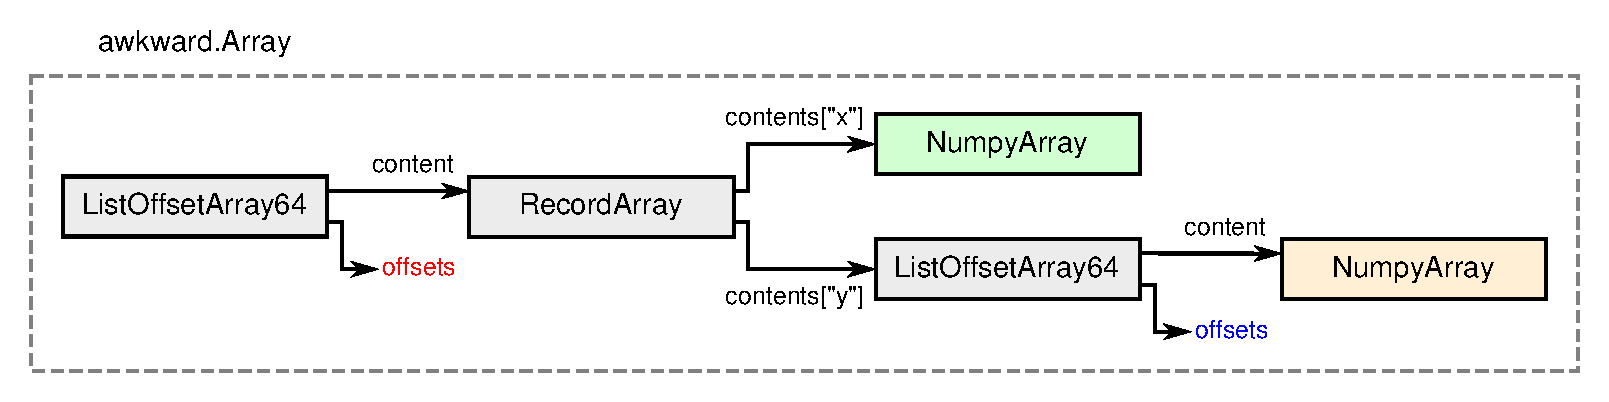
\includegraphics[width=\linewidth]{example-hierarchy.pdf}
\vspace{5 cm}
\end{onlyenv}\begin{onlyenv}<3>
\vspace{0.25 cm}
\begin{minted}{python}
>>> array[:, :, "y", 1:]
\end{minted}

\vspace{0.25 cm}
\begin{Verbatim}[commandchars=\\\{\}]
outer offsets:  \textcolor{red}{0,                     3,  3, 5}
content for x:  \textcolor{darkgreen}{1,  4,      9,            16}
starts  for y:  \textcolor{blue}{0,  1,      3,             6}
stops   for y:  \textcolor{blue}{    1,      3,             6,            10}
content for y: \textcolor{darkorange}{11, 12, 22, 13, 23, 33,    14, 24, 34, 44}
\end{Verbatim}
\vspace{5 cm}
\end{onlyenv}\begin{onlyenv}<4>
\vspace{0.25 cm}
\begin{minted}{python}
>>> array[:, :, "y", 1:]
\end{minted}

\vspace{0.25 cm}
\begin{Verbatim}[commandchars=\\\{\}]
outer offsets:  \textcolor{red}{0,                     3,  3, 5}
content for x:  \textcolor{darkgreen}{1,  4,      9,            16}
starts  for y:  \textcolor{blue}{    1,  2,      4,             7}
stops   for y:  \textcolor{blue}{    1,      3,             6,            10}
content for y: \textcolor{darkorange}{11, 12, 22, 13, 23, 33,    14, 24, 34, 44}
\end{Verbatim}
\vspace{5 cm}
\end{onlyenv}
\end{frame}

\begin{frame}{\only<1>{Awkward 0.x did it with NumPy arrays}\only<2>{Awkward 1.x has a compiled part}\only<3>{But only the low-level kernels {\it must be} compiled}\only<4->{Mid-level Python would make autodiff easier to implement}}
\vspace{0.5 cm}
\only<1>{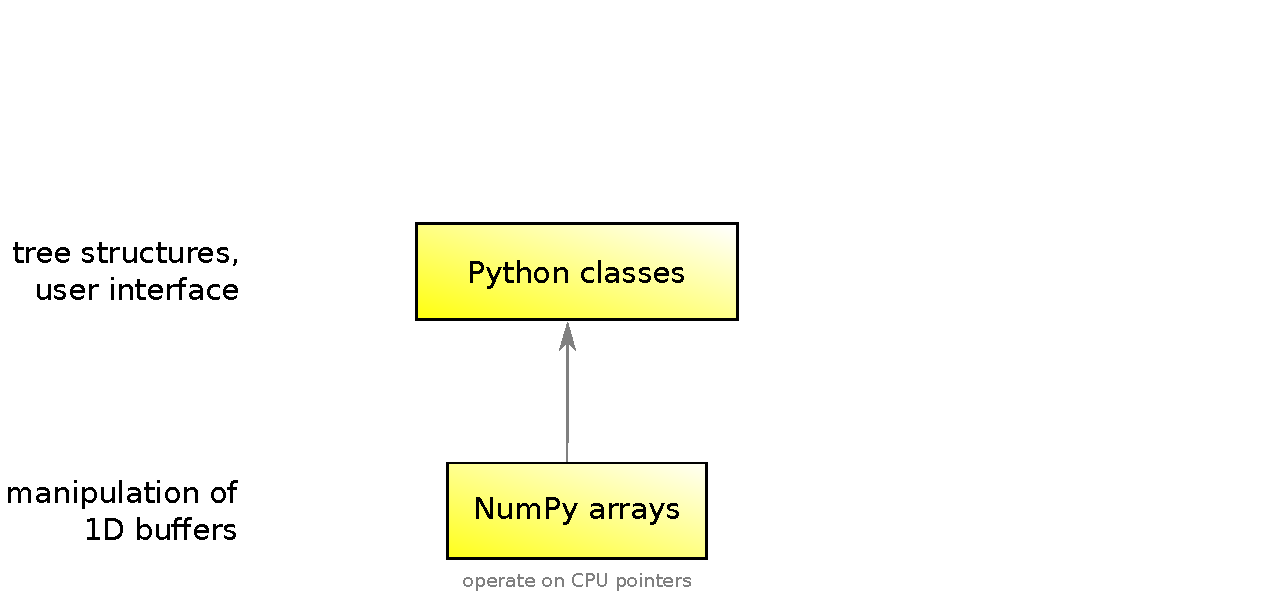
\includegraphics[width=\linewidth]{awkward-1-0-layers-ak0.pdf}}\only<2>{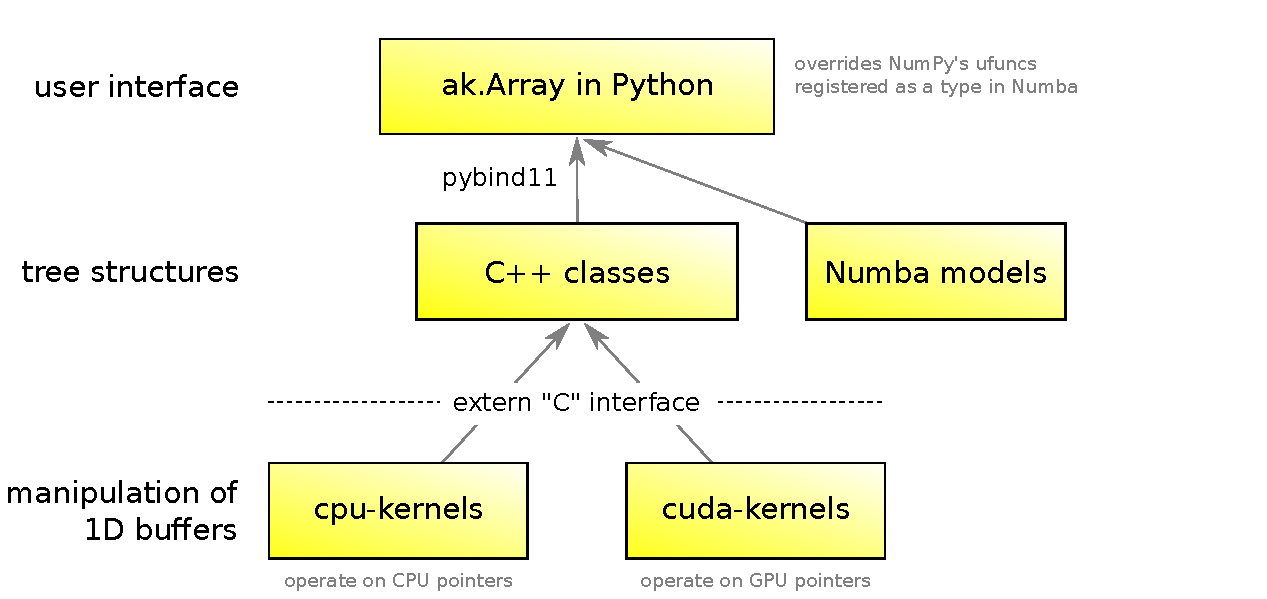
\includegraphics[width=\linewidth]{awkward-1-0-layers-4.pdf}}\only<3>{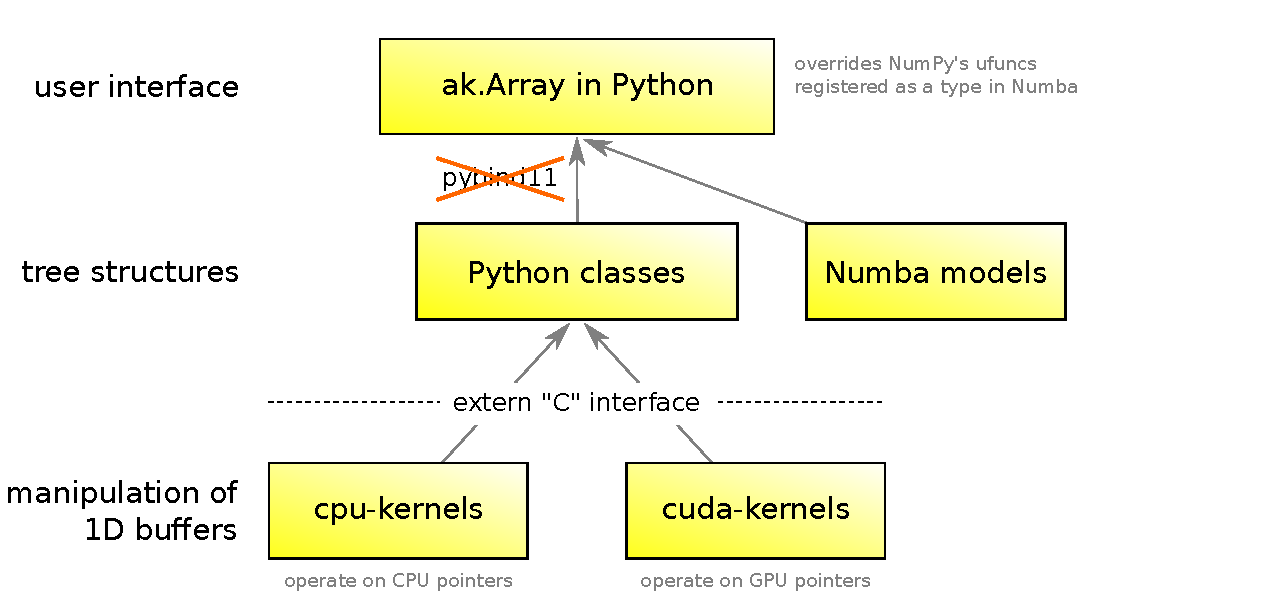
\includegraphics[width=\linewidth]{awkward-1-0-layers-3.pdf}}\only<4>{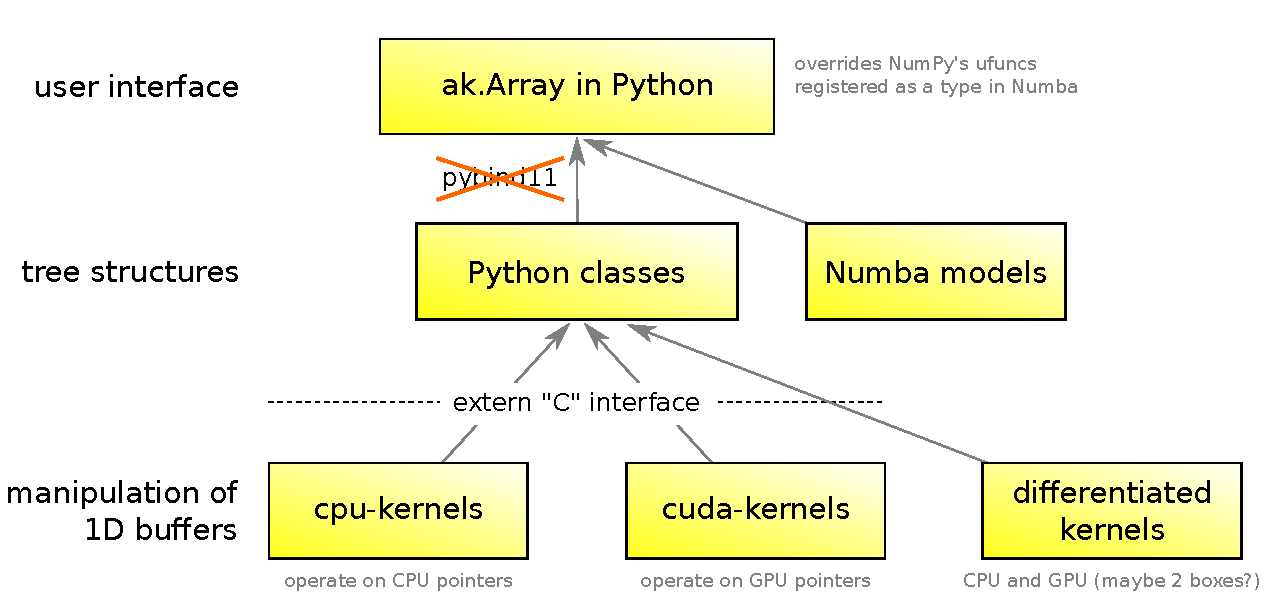
\includegraphics[width=\linewidth]{awkward-1-0-layers-2.pdf}}\only<5>{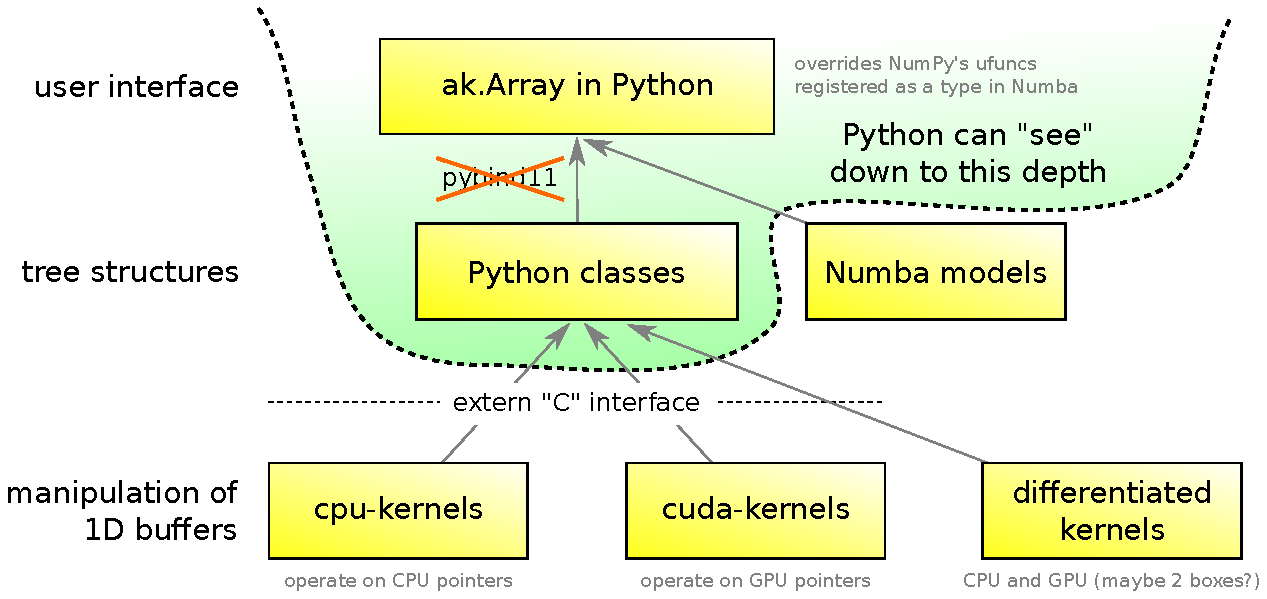
\includegraphics[width=\linewidth]{awkward-1-0-layers-1.pdf}}
\end{frame}

\begin{frame}{Why is this coming up now?}
\vspace{0.25 cm}

\href{https://indico.cern.ch/event/1033648/}{\textcolor{blue}{\underline{Anish put enormous effort}}} into autodifferentiating Awkward Array, but could only handle ufuncs and slices without scalars because of technical issues unrelated to autodifferentiation.

\vspace{0.25 cm}
\hfill 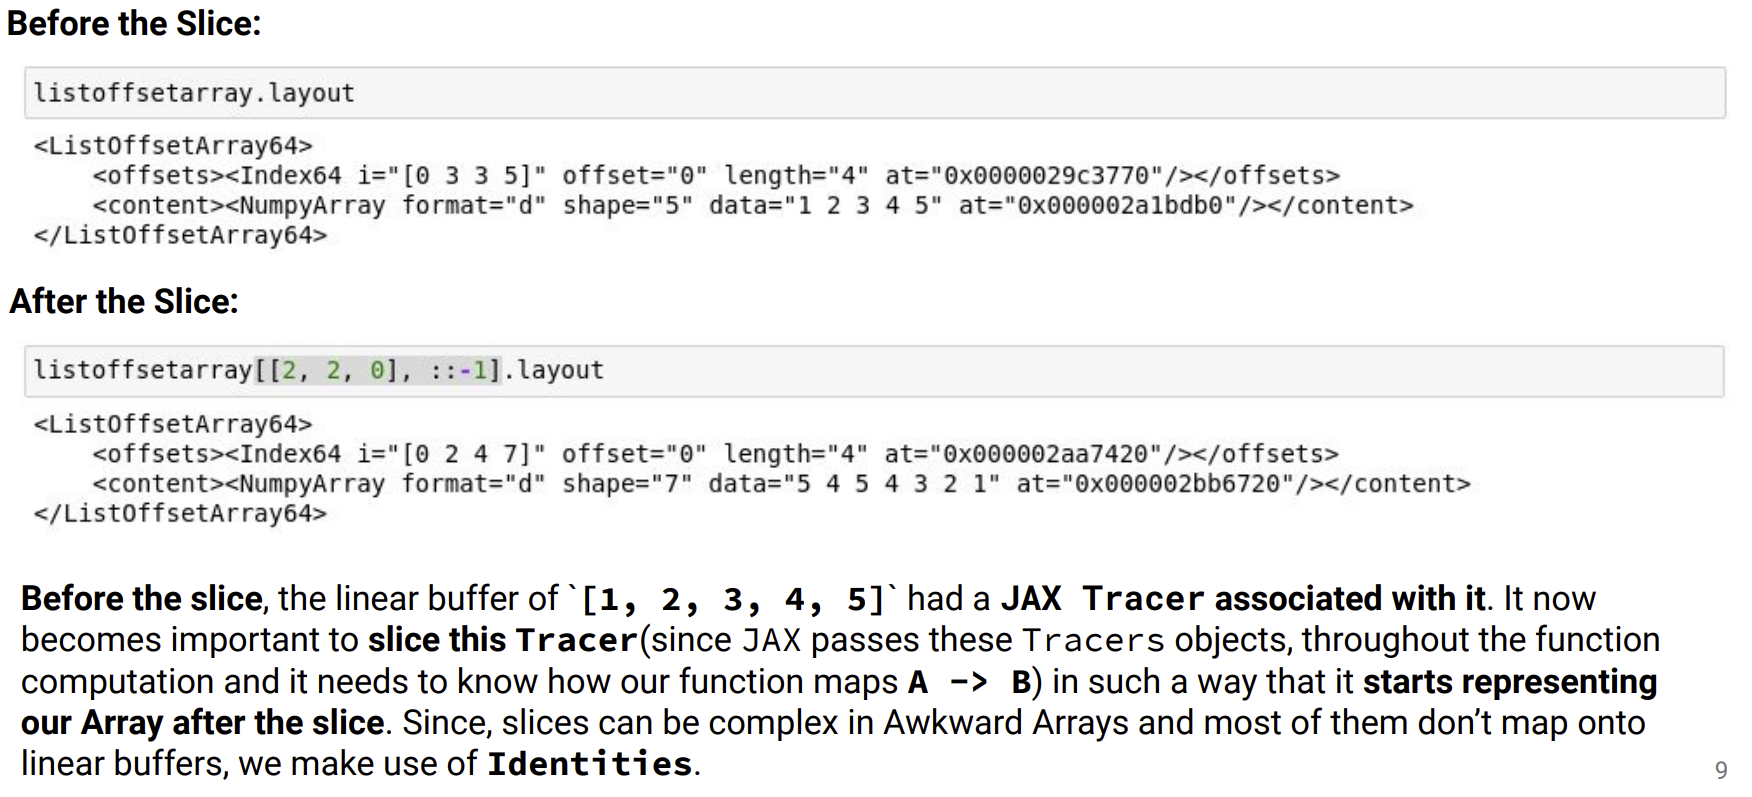
\includegraphics[width=0.9\linewidth]{anish-1.png}
\end{frame}

\begin{frame}{Why is this coming up now?}
\vspace{0.25 cm}

He got around it (for slices with no scalars) by enabling \mintinline{c++}{ak::Identities}, finding out which output corresponds to which input and slicing the JAX Tracers accordingly. This probably isn't generalizable to all Awkward operations.

\vspace{0.25 cm}
\hfill 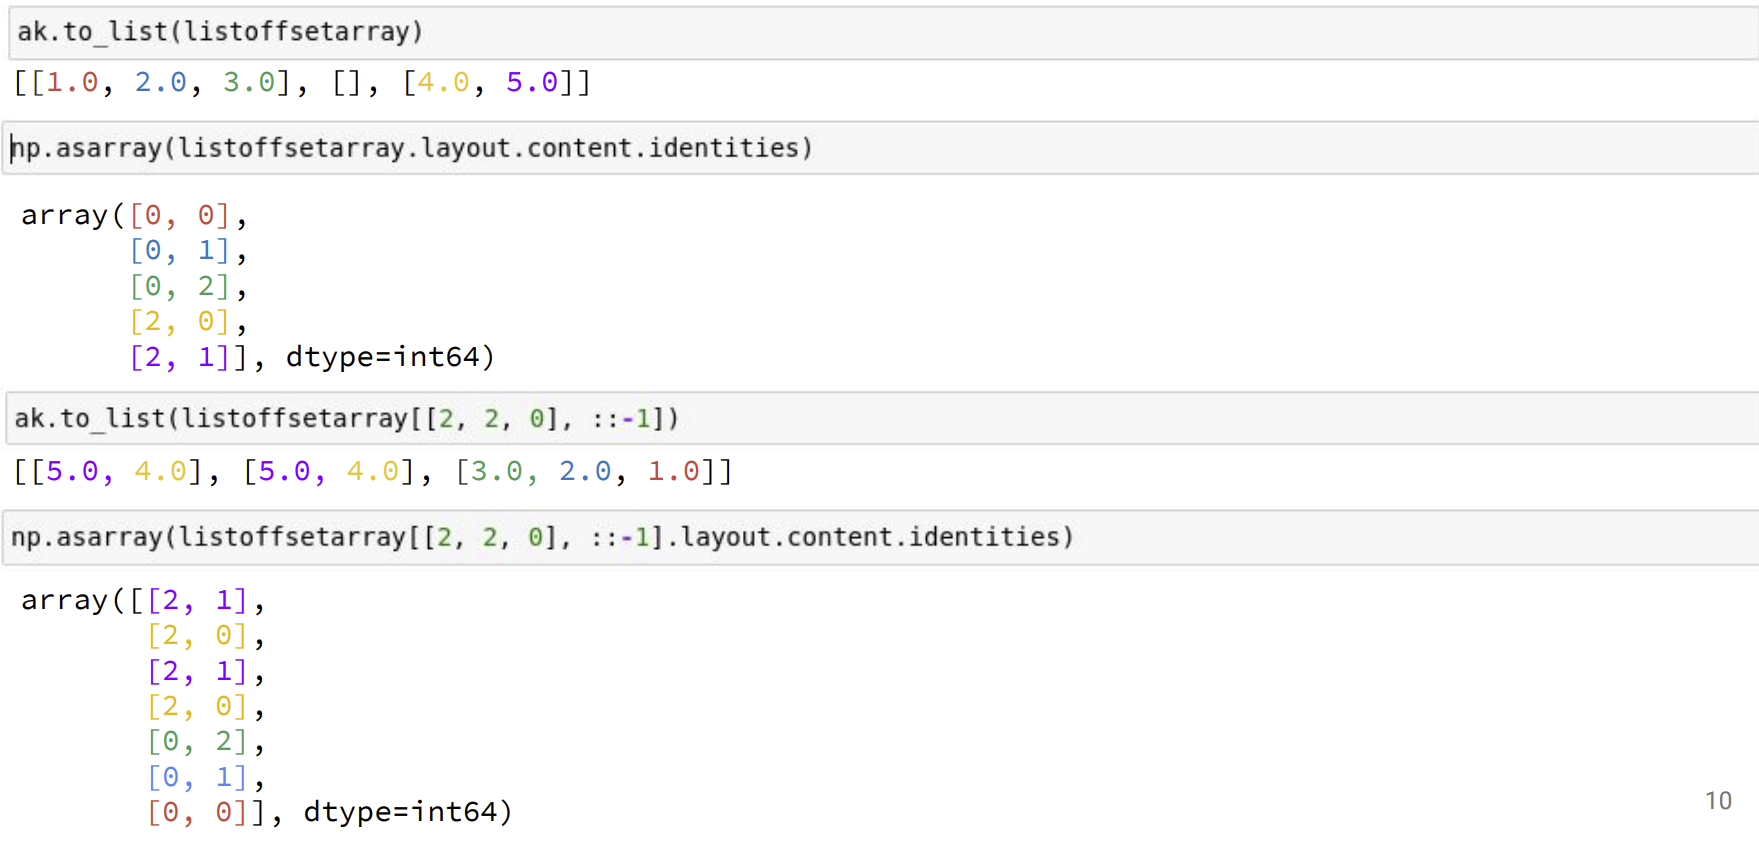
\includegraphics[width=0.9\linewidth]{anish-2.png}
\end{frame}

\begin{frame}{The fundamental problem}
\vspace{0.25 cm}

\only<1>{Ultimately, the problem is that JAX can't ``see'' what happens to 1D arrays. It sees tree structures whose nodes get replaced and 1D buffers get shuffled in complex ways.}\only<2>{But it could be alleviated if JAX could ``see'' down to the level of kernel manipulation. Then it would only need to be told how each kernel shuffles 1D buffers.}\only<3>{Then, Awkward Array would look like an application on arrays (like pyhf) with some extra array-functions we need to tell JAX about (the kernels).}

\vspace{0.1 cm}
\only<1>{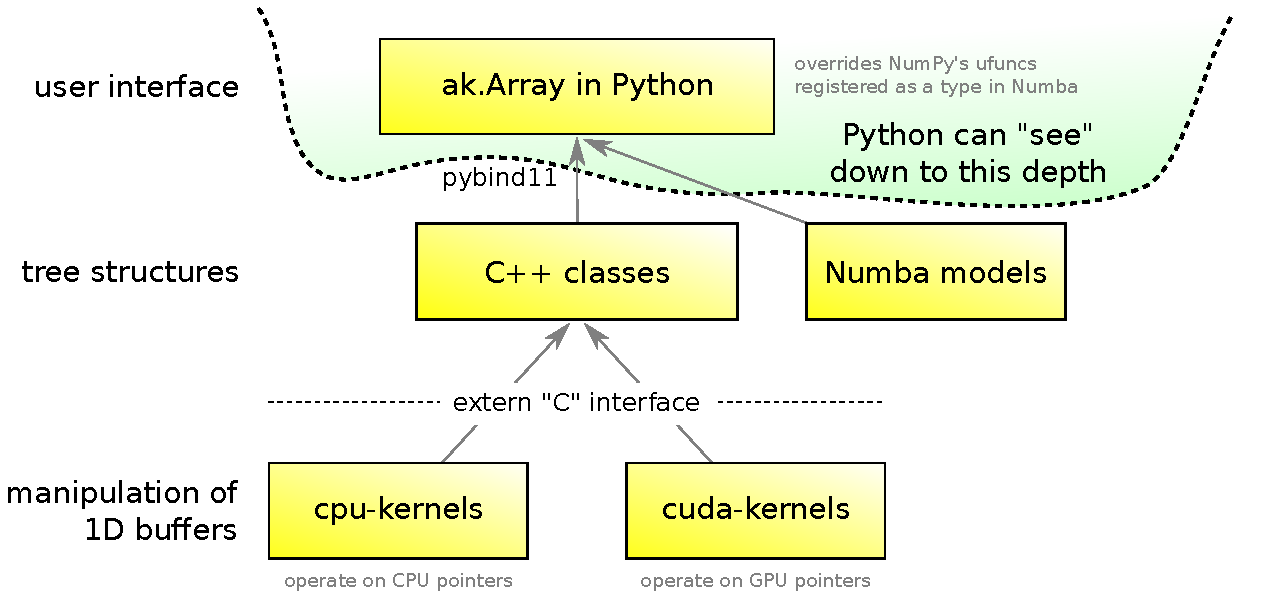
\includegraphics[width=\linewidth]{awkward-1-0-layers-problem.pdf}}\only<2->{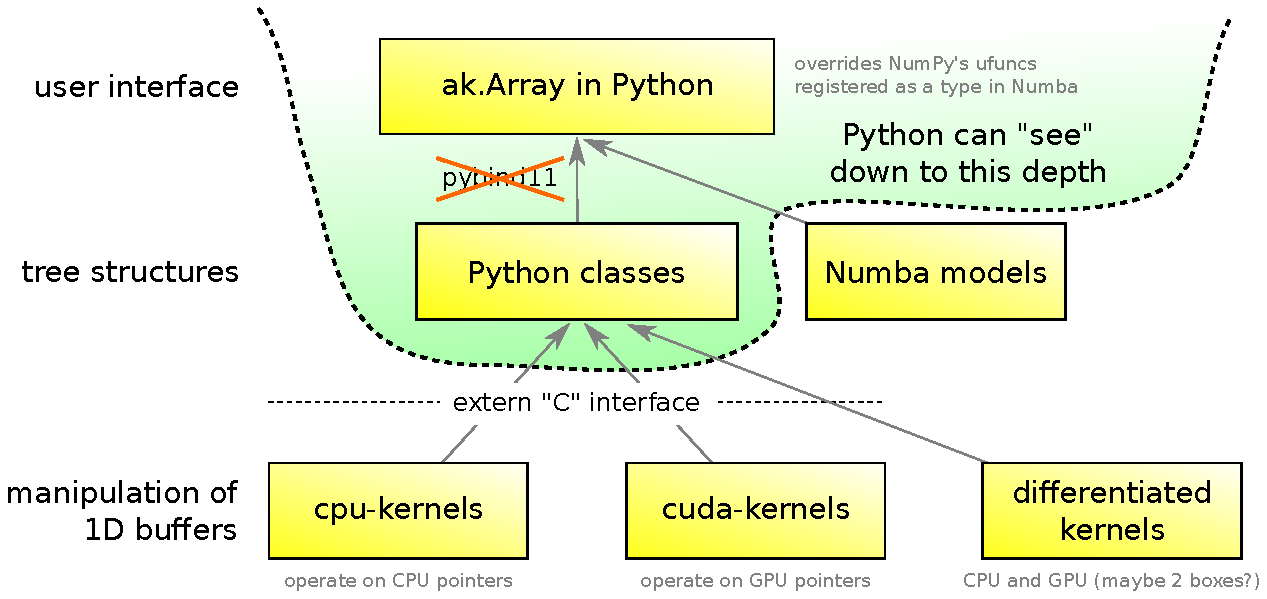
\includegraphics[width=\linewidth]{awkward-1-0-layers-1.pdf}}
\end{frame}

\begin{frame}{It's not just JAX; JAX is what finally convinced me}
\vspace{0.25 cm}
\begin{enumerate}\setlength{\itemsep}{0.35 cm}
\item JAX/autodiff: patched (incompletely) with \mintinline{c++}{ak::Identities}.
\item Garbage collector reference cycles: \mintinline{python}{gc.collect()} can't see cycles that go Python $\to$ C++ $\to$ Python. Patched with \mintinline{python}{weakref} (brittle).
\item Future GPU optimization: to avoid putting unnecessary synchronization points between kernels, we need to give CUDA a DAG of kernels (rather than calling them eagerly). A general way to make such a DAG is with Dask, but only if Dask can see all the way down to the kernel level.
\item Python profilers and debugger: currently, the C++ is opaque. Patched by (manually!) attaching line number references to every exception, but still we don't see the full stack trace.
\item \textcolor{darkorange}{\bf Also, the C++ layer does not serve the function it was created for.}
\end{enumerate}
\end{frame}

\begin{frame}{Why does Awkward Array have a C++ layer?}
\LARGE
\vspace{0.5 cm}

\begin{center}
It is not for performance.
\end{center}

\large
\begin{center}
(The \underline{\it kernels} are compiled for performance; the C++ layer never performs \\ any operations whose time complexity is above $\mathcal{O}(1)$ in array length $n$.)
\end{center}

\LARGE
\vspace{1 cm}
\begin{center}
\uncover<2->{It's for interoperability with C++ libraries.}
\end{center}
\end{frame}

\begin{frame}[fragile]{Quintessential example: bindings to FastJet (C++)}
\large
\vspace{0.5 cm}

The idea was that we would accept many-event sets of particles as jagged record arrays and return many-even sets of jets as jagged record arrays:

\vspace{0.25 cm}
\begin{center}
\begin{minipage}{0.95\linewidth}
\small
\begin{minted}{c++}
ak::Index64 offsets(num_events + 1);
ak::ContentPtr content = std::make_shared<ak::NumpyArray>(...);

// fill offsets and content with jet results

return ak::ListOffsetArray64(offsets, content);
\end{minted}
\end{minipage}
\end{center}

\vspace{0.25 cm}
\uncover<2->{But compiling and linking other projects to Awkward Array is brittle: {\tt \#778}, {\tt \#774}, {\tt \#483}, {\tt \#562}, {\tt \#476}, {\tt \#430}, {\tt \#316}, {\tt \#281}, {\tt \#233}, {\tt \#217}, {\tt \#211}, {\tt \#209}.}

\vspace{0.5 cm}
\uncover<3->{\textcolor{red}{Now that we're actually writing Awkward-FastJet, we're doing it through Python.}}
\end{frame}

\begin{frame}{The \mintinline{python}{ak.from_buffers} function can be a standard interface}
\large
\vspace{0.2 cm}
Any library that can produce a Form (JSON), length (int), and buffers (string names $\to$ 1D buffers map) has effectively produced an Awkward Array.

\vspace{0.2 cm}
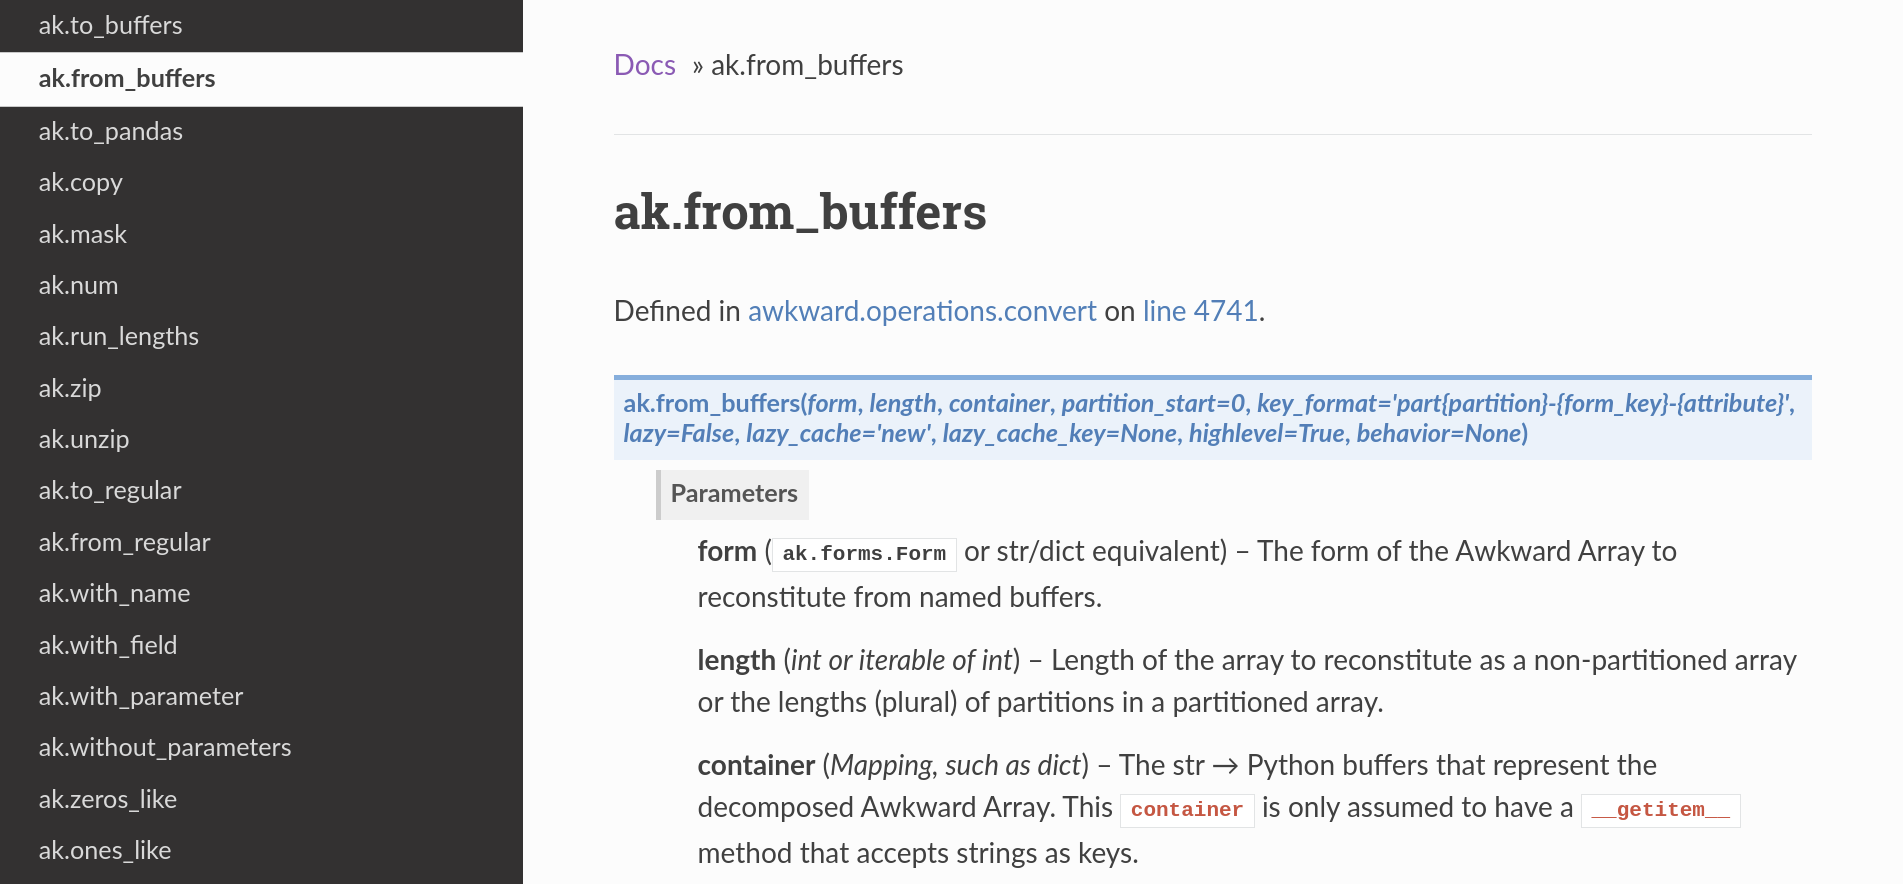
\includegraphics[width=\linewidth]{from_buffers.png}
\end{frame}

\begin{frame}{So this is the plan: zero-interface change refactoring}
\vspace{0.5 cm}
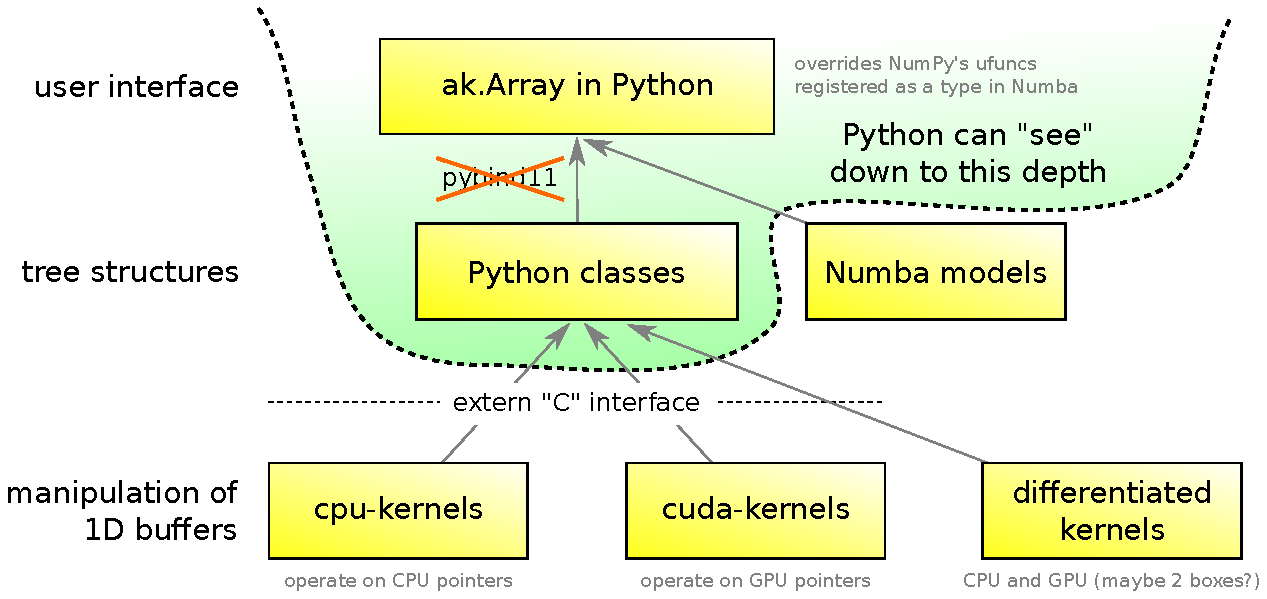
\includegraphics[width=\linewidth]{awkward-1-0-layers-1.pdf}
\end{frame}

\begin{frame}{Ioana Ifrim will be taking it on as a 25\% project, $\sim$6 months}
\vspace{0.4 cm}
\begin{center}
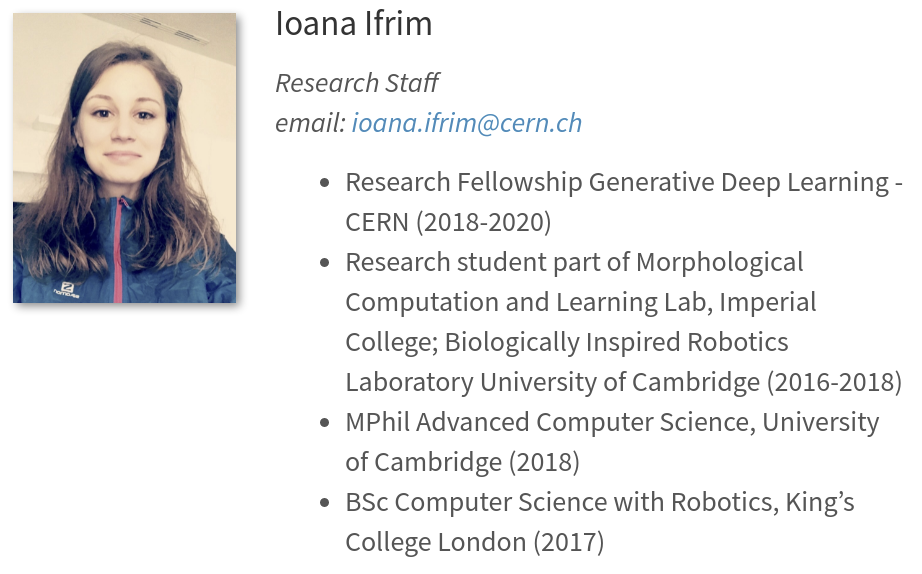
\includegraphics[width=0.8\linewidth]{ioana.png}
\end{center}
\end{frame}

\begin{frame}{Details}
\vspace{0.5 cm}

\begin{itemize}\setlength{\itemsep}{0.5 cm}
\item Not all of the mid-level C++ will be translated. ArrayBuilder, TypedArrayBuilder, and AwkwardForth are not based on kernels and must remain in C++.
\item Therefore, the build procedure will not change (other than the plans Henry has for it already). There will still be a \mintinline{bash}{libawkward.so}, but it will be smaller.
\item 60k lines of C++ will be translated to (maybe) 30k lines of Python.
\item The unit tests that will be needed to compare old C++ and new Python will significantly increase coverage.
\item When we finally remove the old C++, that will be called Awkward 2.0.
\item However, the \underline{\it interface} will not change!
\end{itemize}
\end{frame}

\end{document}
